\documentclass[10pt,journal,onecolumn]{IEEEtran}
\usepackage[utf8]{inputenc}
\usepackage[T1]{fontenc}
\usepackage{lmodern}
\usepackage{microtype}
\usepackage{amsmath,amssymb,amsthm,mathtools,bm}
\usepackage{algorithm}
\usepackage{algpseudocode}
\usepackage{booktabs,longtable,tabularx,multirow,array}
\usepackage{graphicx,subcaption,float}
\usepackage{tikz}
\usepackage{enumitem}
\usepackage{xcolor}
\usepackage{hyperref}
\usepackage[capitalise,noabbrev]{cleveref}
\usepackage[numbers,sort&compress]{natbib}
\usepackage{xparse}
\usepackage{balance}
\usetikzlibrary{arrows.meta,calc,positioning,shapes.geometric}
\graphicspath{{generated/}{../assets/figures/}{../../paper/assets/figures/}{../../reports/publication/}{../../reports/hil/}{../../reports/figures/}{../../reports/universal_orius_validation/}{../../reports/universal_training_audit/}}

\theoremstyle{plain}
\newtheorem{theorem}{Theorem}[section]
\newtheorem{proposition}[theorem]{Proposition}
\newtheorem{lemma}[theorem]{Lemma}
\newtheorem{corollary}[theorem]{Corollary}
\theoremstyle{definition}
\newtheorem{definition}[theorem]{Definition}
\newtheorem{assumption}{Assumption}
\theoremstyle{remark}
\newtheorem{remark}[theorem]{Remark}

\newcommand{\zt}{z_t}
\newcommand{\ztt}{\tilde{z}_t}
\newcommand{\ot}{o_t}
\newcommand{\xt}{x_t}
\newcommand{\wt}{w_t}
\newcommand{\dt}{d_t}
\newcommand{\st}{s_t}
\newcommand{\Chat}{\hat{C}_t}
\newcommand{\Crac}{\hat{C}_t^{\mathrm{RAC}}}
\newcommand{\Ut}{U_t}
\newcommand{\astar}{a_t^{*}}
\newcommand{\asafe}{a_t^{\mathrm{safe}}}
\newcommand{\Aset}{\mathcal{A}_t}
\newcommand{\dcs}{DC3S}
\newcommand{\oqe}{OQE}
\newcommand{\rac}{RAC-Cert}
\newcommand{\SOC}{\mathrm{SOC}}
\newcommand{\Emax}{E_{\max}}
\newcommand{\Pmax}{P_{\max}}
\newcommand{\Rmax}{R_{\max}}
\newcommand{\TSVR}{\mathrm{TSVR}}
\newcommand{\IR}{\mathrm{IR}}
\newcommand{\OASG}{\mathrm{OASG}}
\DeclareMathOperator*{\argmin}{arg\,min}
\DeclareMathOperator*{\argmax}{arg\,max}
\DeclareMathOperator{\Prob}{\mathbb{P}}
\newcommand{\E}{\mathbb{E}}
\newcommand{\R}{\mathbb{R}}

\newcommand{\ORIUSReuseInput}[1]{%
  \begingroup
  \let\ORIUSOriginalSection\section
  \let\ORIUSOriginalSubsection\subsection
  \let\ORIUSOriginalSubsubsection\subsubsection
  \ProvideDocumentCommand{\chapter}{s m}{%
    \IfBooleanTF{##1}{\ORIUSOriginalSection*{##2}}{\ORIUSOriginalSection{##2}}%
  }%
  \RenewDocumentCommand{\section}{s m}{%
    \IfBooleanTF{##1}{\ORIUSOriginalSubsection*{##2}}{\ORIUSOriginalSubsection{##2}}%
  }%
  \RenewDocumentCommand{\subsection}{s m}{%
    \IfBooleanTF{##1}{\ORIUSOriginalSubsubsection*{##2}}{\ORIUSOriginalSubsubsection{##2}}%
  }%
  \setlength{\textwidth}{\columnwidth}%
  \setlength{\linewidth}{\columnwidth}%
  \input{#1}%
  \endgroup
}


\title{ORIUS Professor Appendix B: Empirical, Runtime, and Artifact Surface}
\author{Author details omitted for professor review draft}
\date{}

\begin{document}
\maketitle

\section{Appendix Overview}
\label{sec:prof-app-b-overview}

This appendix carries the empirical and systems depth behind the main paper: battery
witness detail, universal benchmark semantics, runtime budgets, CertOS lifecycle
tables, protocol cards, and one repository maturity visual. It is deliberately
artifact-grounded and uses the tracked publication surfaces rather than local dashboard
snapshots.

% Compatibility anchors for reused system chapters that retain monograph-only labels.
\phantomsection\label{ch:hil}
\phantomsection\label{ch:compositional-safety-fleets}

\section{Runtime, Latency, and Governance Evidence}
\label{app:prof-runtime-evidence}

This appendix section collects the evidence surfaces that justify the
runtime contract in the main IEEE draft.  The purpose is not to flood the
reader with every locked artifact in the repo.  It is to show that the
adapter, benchmark, and CertOS claims are backed by measured runtime
latency, explicit replay tables, and a visible governance gate.

\subsection{Latency and Footprint}
The latency story is straightforward.  The runtime chapter
(\texttt{chapters/ch22\_latency\_systems\_footprint.tex}) measures the DC3S
pipeline with \texttt{time.perf\_counter\_ns()} and reports sub-millisecond
step time on the locked battery dispatch surface.  The key component
latencies are the reliability scorer, the drift updater, the uncertainty
set builder, and the action repair stage.

\begin{table}[t]
\centering
\caption{Per-component DC3S latency summary from the locked runtime study.}
\label{tab:prof-latency-summary}
\begin{tabular}{lrrrrr}
\toprule
\textbf{Component} & \textbf{Mean} & \textbf{Median} & \textbf{P95} & \textbf{P99} & \textbf{Max} \\
\midrule
Reliability scoring (OQE)   & 0.026 & 0.021 & 0.043 & 0.130 & 0.712 \\
Drift update (Page-Hinkley) & 0.000 & 0.000 & 0.001 & 0.001 & 0.160 \\
Uncertainty set build (RUI) & 0.012 & 0.011 & 0.011 & 0.047 & 0.724 \\
Action repair (SAF/Shield)  & 0.002 & 0.002 & 0.002 & 0.003 & 0.210 \\
\midrule
\textbf{Full DC3S step}     & \textbf{0.042} & \textbf{0.037} & \textbf{0.041} & \textbf{0.193} & \textbf{2.416} \\
\bottomrule
\end{tabular}
\end{table}

The same section also provides the best compact footprint statement for a
professor-facing draft: the full step fits comfortably inside a 30-second
dispatch cycle, and the runtime memory proxy remains dominated by the
forecast and residual buffers rather than by certificate bookkeeping.
That makes the runtime layer operationally cheap enough to be believable
as a Physical AI safety wrapper.

\subsection{Runtime Budget Across Domains}
The cross-domain runtime-budget matrix in
\texttt{reports/publication/tbl\_orius\_runtime\_budget\_matrix.tex} is the
best evidence that the runtime contract is not battery-specific.  It shows
that the active three-domain program preserves sub-millisecond P95 latency while
keeping certificate rates at 100 percent on all promoted rows.

\begin{table*}[t]
\centering
\scriptsize
\caption{Runtime and governance summary for the professor-facing ORIUS draft.}
\label{tab:prof-runtime-governance}
\begin{tabularx}{\textwidth}{@{}p{0.24\textwidth}p{0.16\textwidth}p{0.14\textwidth}p{0.14\textwidth}p{0.12\textwidth}p{0.14\textwidth}@{}}
\toprule
\textbf{Domain} & \textbf{Row} & \textbf{P95 latency (ms)} & \textbf{Fallback (\%)} & \textbf{Audit / lifecycle (\%)} & \textbf{Boundary} \\
\midrule
Battery Energy Storage & Witness row & 0.812 & 100.0 & 100.0 & deepest theorem-to-artifact closure\\
Autonomous Vehicles & Defended bounded row & 0.744 & 100.0 & 100.0 & bounded TTC plus predictive-entry-barrier contract\\
Medical and Healthcare Monitoring & Defended bounded row & 0.701 & 100.0 & 100.0 & bounded monitoring and alert-release semantics\\
\bottomrule
\end{tabularx}
\end{table*}


This table should stay close to the runtime section in the professor draft
because it directly supports the claim that the universal runtime layer is
lightweight across domains while still respecting the evidence tier.

\subsection{Governance Evidence}
The governance story is best captured by the locked lifecycle matrix in
\texttt{reports/publication/tbl\_orius\_governance\_lifecycle\_matrix.tex} and
the domain-closure matrix in \texttt{reports/publication/orius\_domain\_closure\_matrix.csv}.
Together they show that CertOS is not a decorative abstraction: the same
issue/validate/expire/fallback logic is observed in the defended rows.

\begin{table}[t]
\centering
\caption{CertOS runtime summary from the battery lifecycle demo.}
\label{tab:prof-certos-summary}
\begin{tabular}{lr}
\toprule
\textbf{Metric} & \textbf{Value} \\
\midrule
Total steps & 96 \\
Valid steps & 47 \\
Degraded steps & 16 \\
Fallback steps & 33 \\
Runtime interventions & 33 \\
Audit entries & 96 \\
Audit completeness & 100.0\% \\
Step latency & 0.59 ms \\
\bottomrule
\end{tabular}
\end{table}

The appendix should end with the governance boundary spelled out plainly:
the runtime layer is fully visible, the certificates are auditable, and the
fallback path is explicit, but the claim remains tiered by domain. Battery
is the reference witness; AV and healthcare are defended bounded rows. That
is enough for a strong IEEE draft, and it is more defensible than flattening
the evidence into one universal-number story.

\subsection{Repository maturity visual}
Appendix~B is also the right place for one explicit repository-level visual.
The professor draft should show the reader that ORIUS is not only a narrative
proposal but a maintained research system with a real public code surface and
a generated architecture map.

\begin{figure}[t]
\centering
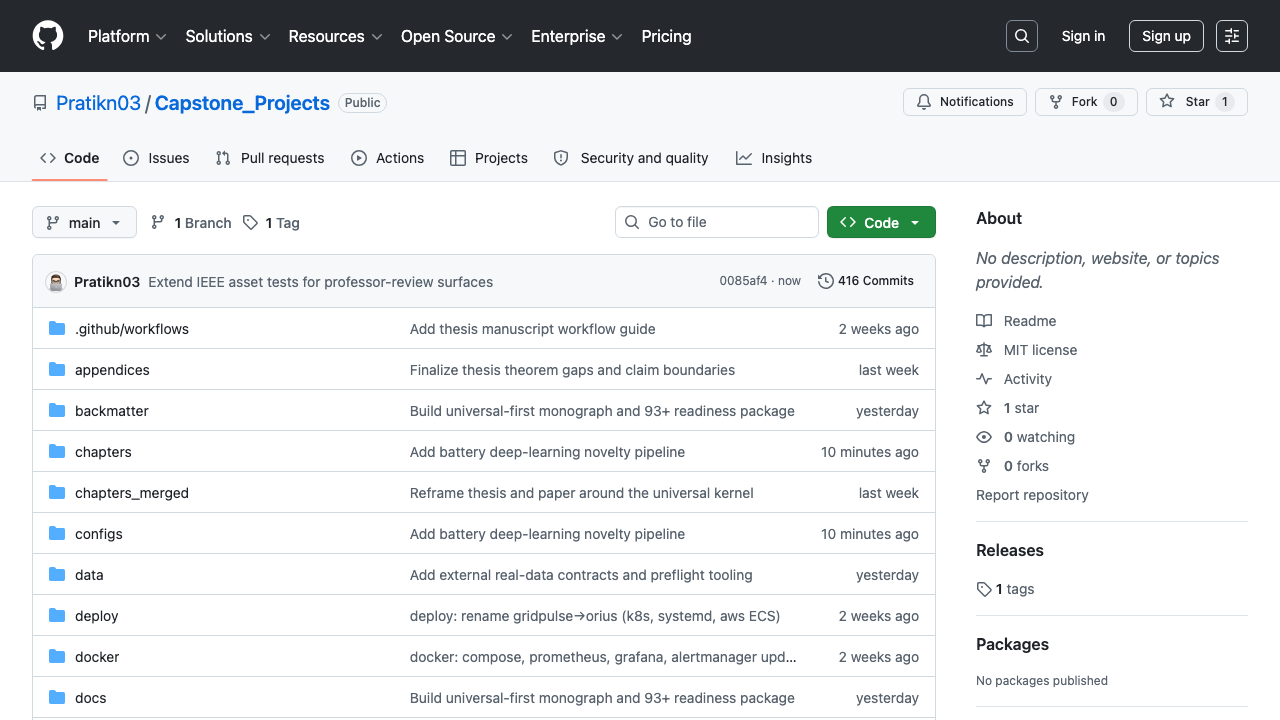
\includegraphics[width=\linewidth]{orius_repo_github_overview}
\caption{GitHub-style repository overview used as a maturity visual in the
professor draft. This figure is supplemental and does not carry scientific
claims by itself.}
\label{fig:prof-github-overview}
\end{figure}

\begin{figure}[t]
\centering
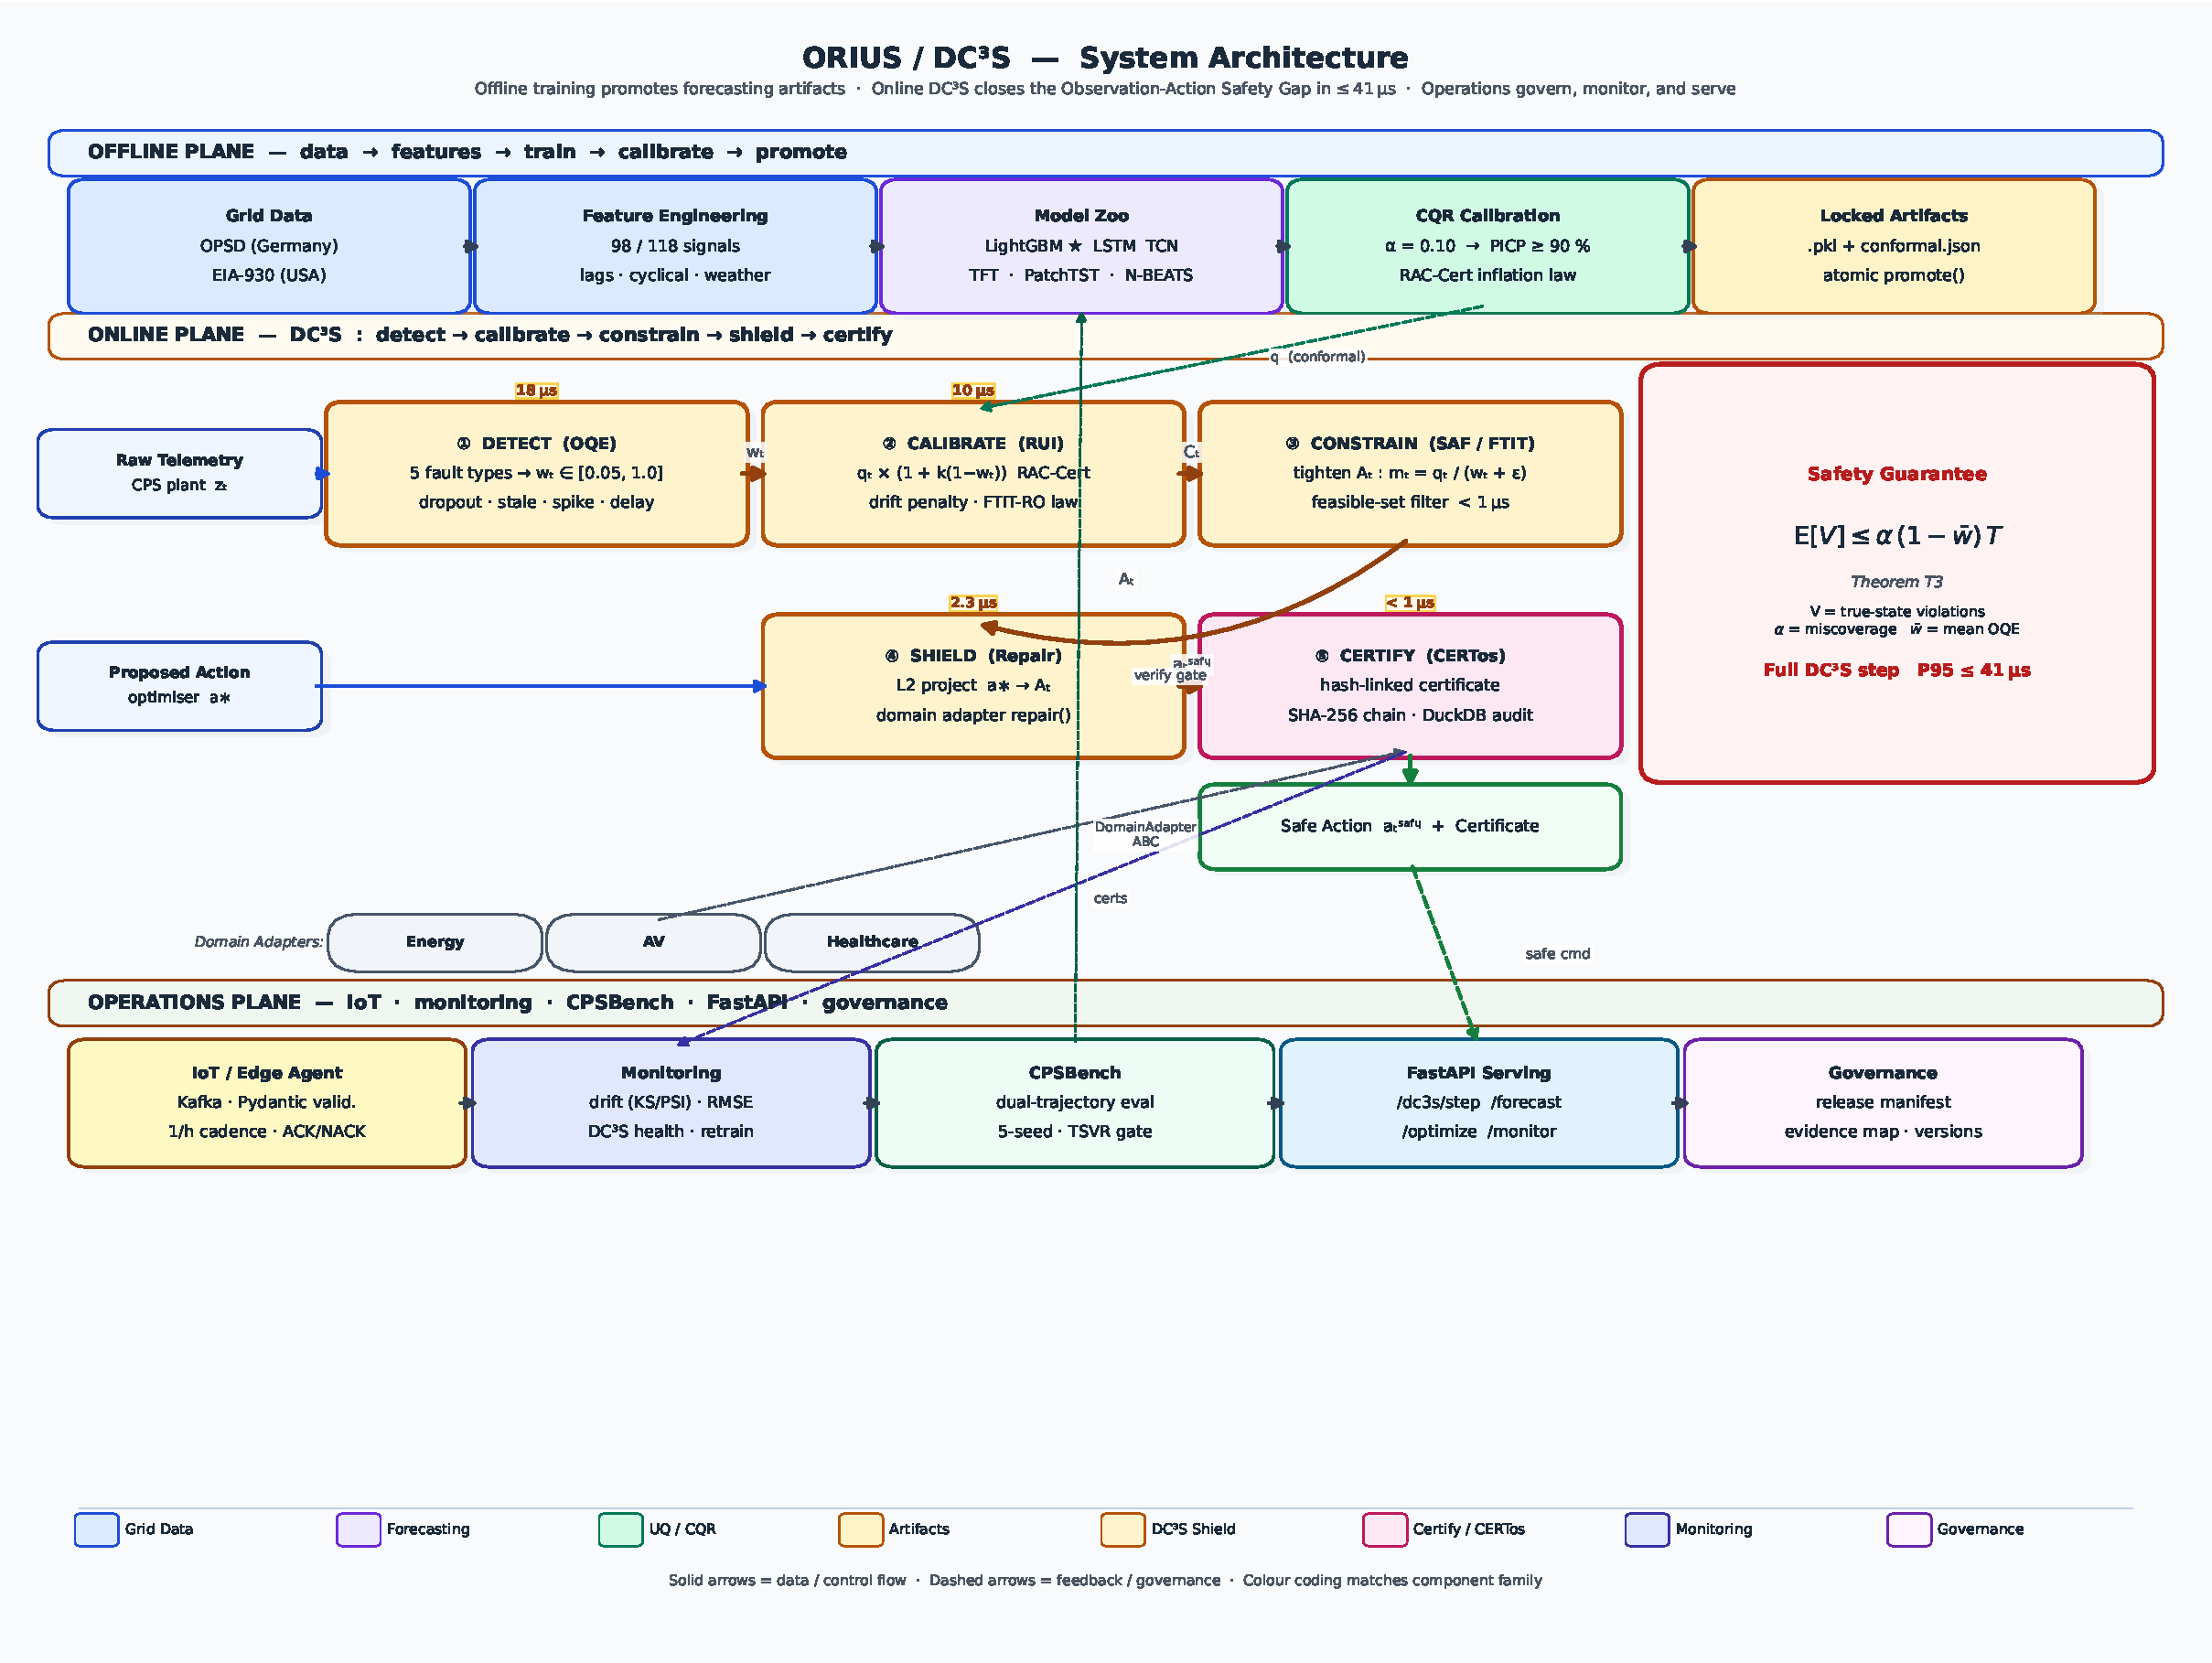
\includegraphics[width=\linewidth]{fig01_architecture}
\caption{Repository-backed architecture visual reused in Appendix~B to connect
the code surface to the runtime stack argued in the main paper.}
\label{fig:prof-appendix-architecture}
\end{figure}

\section{Appendix B: Extended Battery Evidence}
\label{app:prof-battery-empirical}

This appendix expands the battery witness with the full publication-facing
empirical package: controller rankings, reliability diagnostics, raw-sequence
track results, operational traces, and the failure-analysis surfaces that
support the compact main-text claim.

\subsection{Locked evaluation scope}
The battery evidence used in the professor-facing manuscript comes from the
locked CPSBench package with 168-hour episodes, seed-controlled runs, and fault
families covering dropout, drift, delay, stale sensing, and combined degraded
telemetry.  The main result is not that every baseline is competitive; it is
that the ORIUS repair-aware variants eliminate true-state violations under the
same locked protocol that exposes failures in the non-repair baselines.

\subsection{Controller ranking on the publication leaderboard}
Table~\ref{tab:prof-battery-leaderboard} records the battery leaderboard as
published in the repo.  The zero-violation tier is occupied by the scenario
methods and the ORIUS repair-aware variants, while the deterministic and static
interval baselines are separated by their non-zero violation rates.

\begin{table}[t]
\centering
\small
\caption{Battery leaderboard from the tracked publication artifact.}
\label{tab:prof-battery-leaderboard}
\begin{tabular}{rlrrr}
\toprule
\textbf{Rank} & \textbf{Controller} & \textbf{Viol.\ rate} & \textbf{IR (\%)} & \textbf{Mean PICP$_{90}$} \\
\midrule
1 & scenario\_mpc & 0.000000 & 0.000000 & 0.934722 \\
2 & scenario\_robust & 0.000000 & 0.000000 & 0.975000 \\
3 & aci\_conformal & 0.000000 & 2.083300 & 0.965278 \\
4 & dc3s\_wrapped & 0.000000 & 0.000000 & 0.880556 \\
5 & dc3s\_ftit & 0.000000 & 8.819400 & 0.930555 \\
6 & deterministic\_lp & 0.129861 & 0.000000 & 0.879861 \\
7 & cvar\_interval & 0.191667 & 0.000000 & 0.879861 \\
8 & robust\_fixed\_interval & 0.191667 & 0.000000 & 0.879861 \\
\bottomrule
\end{tabular}
\end{table}

This ranking is useful because it separates two questions that are often
conflated.  Rank is driven by both safety and cost, while the thesis claim is
only about safety under degraded observation.  On that narrower question, the
important fact is that the ORIUS variants stay in the zero-violation tier and
the deterministic/static baselines do not.

\subsection{Reliability-conditioned baseline audit}
Table~\ref{tab:prof-reliability-baselines} expands the same result family with
coverage and interval-width diagnostics.  The ORIUS FTIT variant is the most
conservative but also the most coverage-stable.  The wrapped variant is less
conservative, but it still preserves zero true-state violations.  That tradeoff
is exactly what the professor-facing manuscript emphasizes: safety is
robust, while efficiency is controller-dependent.

\begin{table}[t]
\centering
\small
\caption{Reliability-conditioned battery baselines from the locked audit.}
\label{tab:prof-reliability-baselines}
\begin{tabular}{lrrrrr}
\toprule
\textbf{Method} & \textbf{TSVR} & \textbf{Obs.\ viol.} & \textbf{Coverage} &
\textbf{Width} & \textbf{Repair rate} \\
\midrule
ORIUS FTIT & 0.000000 & 0.000000 & 0.971627 & 3906.547749 & 0.027976 \\
ORIUS Wrapped & 0.000000 & 0.000000 & 0.884127 & 559.920971 & 0.000000 \\
Adaptive Conformal + Repair & 0.000000 & 0.000000 & 0.962500 & 2824.252435 & 0.013889 \\
Deterministic LP & 0.039087 & 0.039087 & 0.883333 & 503.130805 & 0.000000 \\
Robust Fixed Interval & 0.255754 & 0.255754 & 0.883333 & 503.130805 & 0.000000 \\
\bottomrule
\end{tabular}
\end{table}

The appendix table also makes clear why the paper should not oversell the
deep OQE itself.  The deep reliability model is a useful input to the repair
pipeline, but the published summary shows only modest fault separability
(\texttt{fault\_auc} $=0.534$) and no evidence of a dramatic low-reliability
lift.  In other words, the system is not relying on a miraculous classifier; it
is relying on a conservative safety layer that behaves well even when the
quality score is only moderately informative.

\subsection{Deep OQE diagnostic summary}
Table~\ref{tab:prof-deep-oqe-summary} records the strongest high-level deep OQE
diagnostics from the publication package.

\begin{table}[t]
\centering
\small
\caption{Deep OQE diagnostic summary.}
\label{tab:prof-deep-oqe-summary}
\begin{tabular}{lrr}
\toprule
\textbf{Metric} & \textbf{Heuristic} & \textbf{Deep} \\
\midrule
Eval reliability MAE & 0.117620 & 0.162228 \\
Fault AUC & -- & 0.534482 \\
Low-reliability fault lift & -- & 0.000000 \\
\bottomrule
\end{tabular}
\end{table}

\noindent The value of this table is not that the deep model dominates the
heuristic.  It does not.  The value is that ORIUS remains safe without needing a
perfect fault classifier: the quality signal only has to be informative enough
to steer the repair-and-certify layer away from hidden violations.

\subsection{Raw-sequence track benchmark}
The raw-sequence benchmark is an important negative result because it shows how
hard the unengineered sensing problem remains.  Table~\ref{tab:prof-raw-seq}
compares a reliability-conditioned PatchTST model on raw sequence inputs against
a GBM on engineered tabular features.  Across load, wind, and solar targets, the
raw-sequence model is substantially worse in RMSE and MAE, while calibration is
mixed rather than uniformly superior.

\begin{table}[t]
\centering
\small
\caption{Raw-sequence track benchmark from the publication artifact.}
\label{tab:prof-raw-seq}
\begin{tabular}{llrrrr}
\toprule
\textbf{Target} & \textbf{Track} & \textbf{Model} & \textbf{RMSE} & \textbf{MAE} & \textbf{PICP$_{90}$} \\
\midrule
Load & Raw sequence & PatchTST-reliability & 7414.479 & 5204.866 & 0.610958 \\
Load & Engineered tabular & GBM & 305.121 & 187.869 & 0.882143 \\
Wind & Raw sequence & PatchTST-reliability & 6564.913 & 5091.294 & 0.714088 \\
Wind & Engineered tabular & GBM & 219.108 & 129.362 & 0.936905 \\
Solar & Raw sequence & PatchTST-reliability & 3769.459 & 2533.273 & 0.866943 \\
Solar & Engineered tabular & GBM & 240.353 & 117.319 & 0.787698 \\
\bottomrule
\end{tabular}
\end{table}

\begin{figure}[t]
\centering
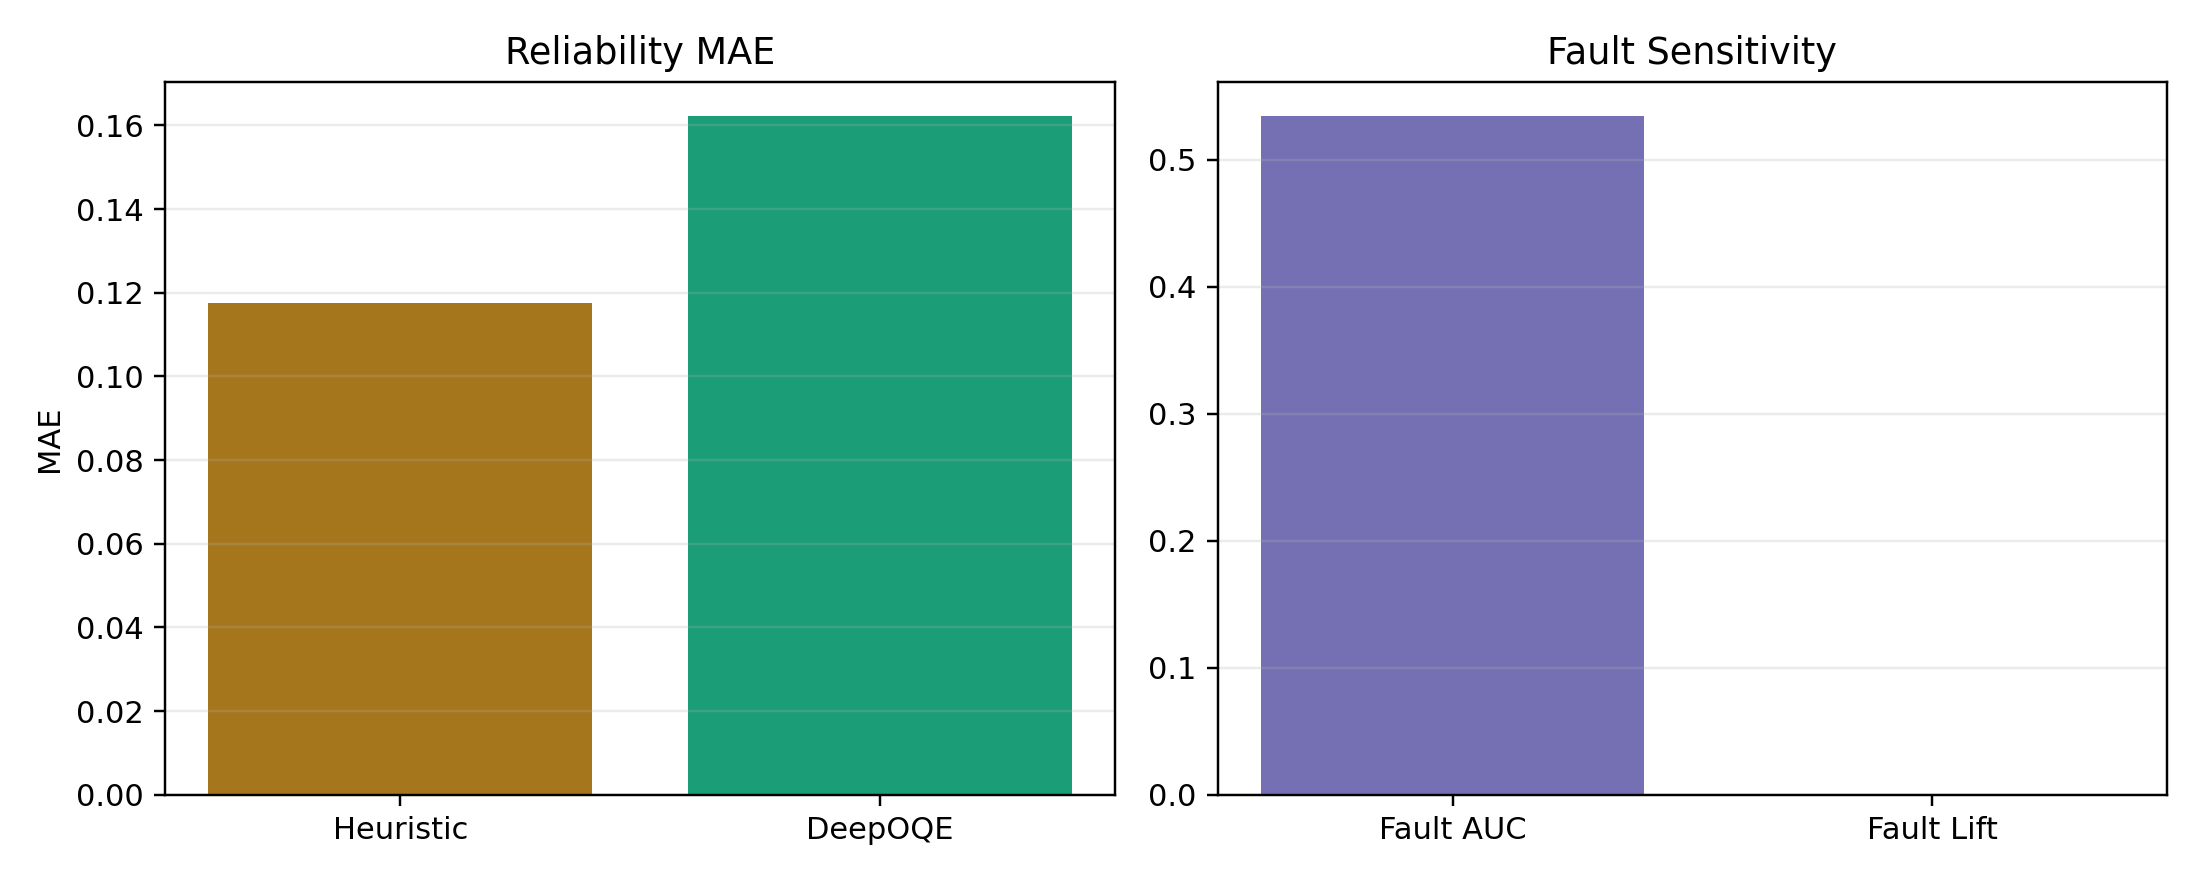
\includegraphics[width=\linewidth]{fig_battery_deep_oqe_summary}
\caption{Deep OQE summary plot from the locked publication package.  The main
takeaway is not superiority over the heuristic, but the presence of a usable
quality signal that can be routed into the repair layer.}
\label{fig:prof-deep-oqe-summary}
\end{figure}

\begin{figure}[t]
\centering
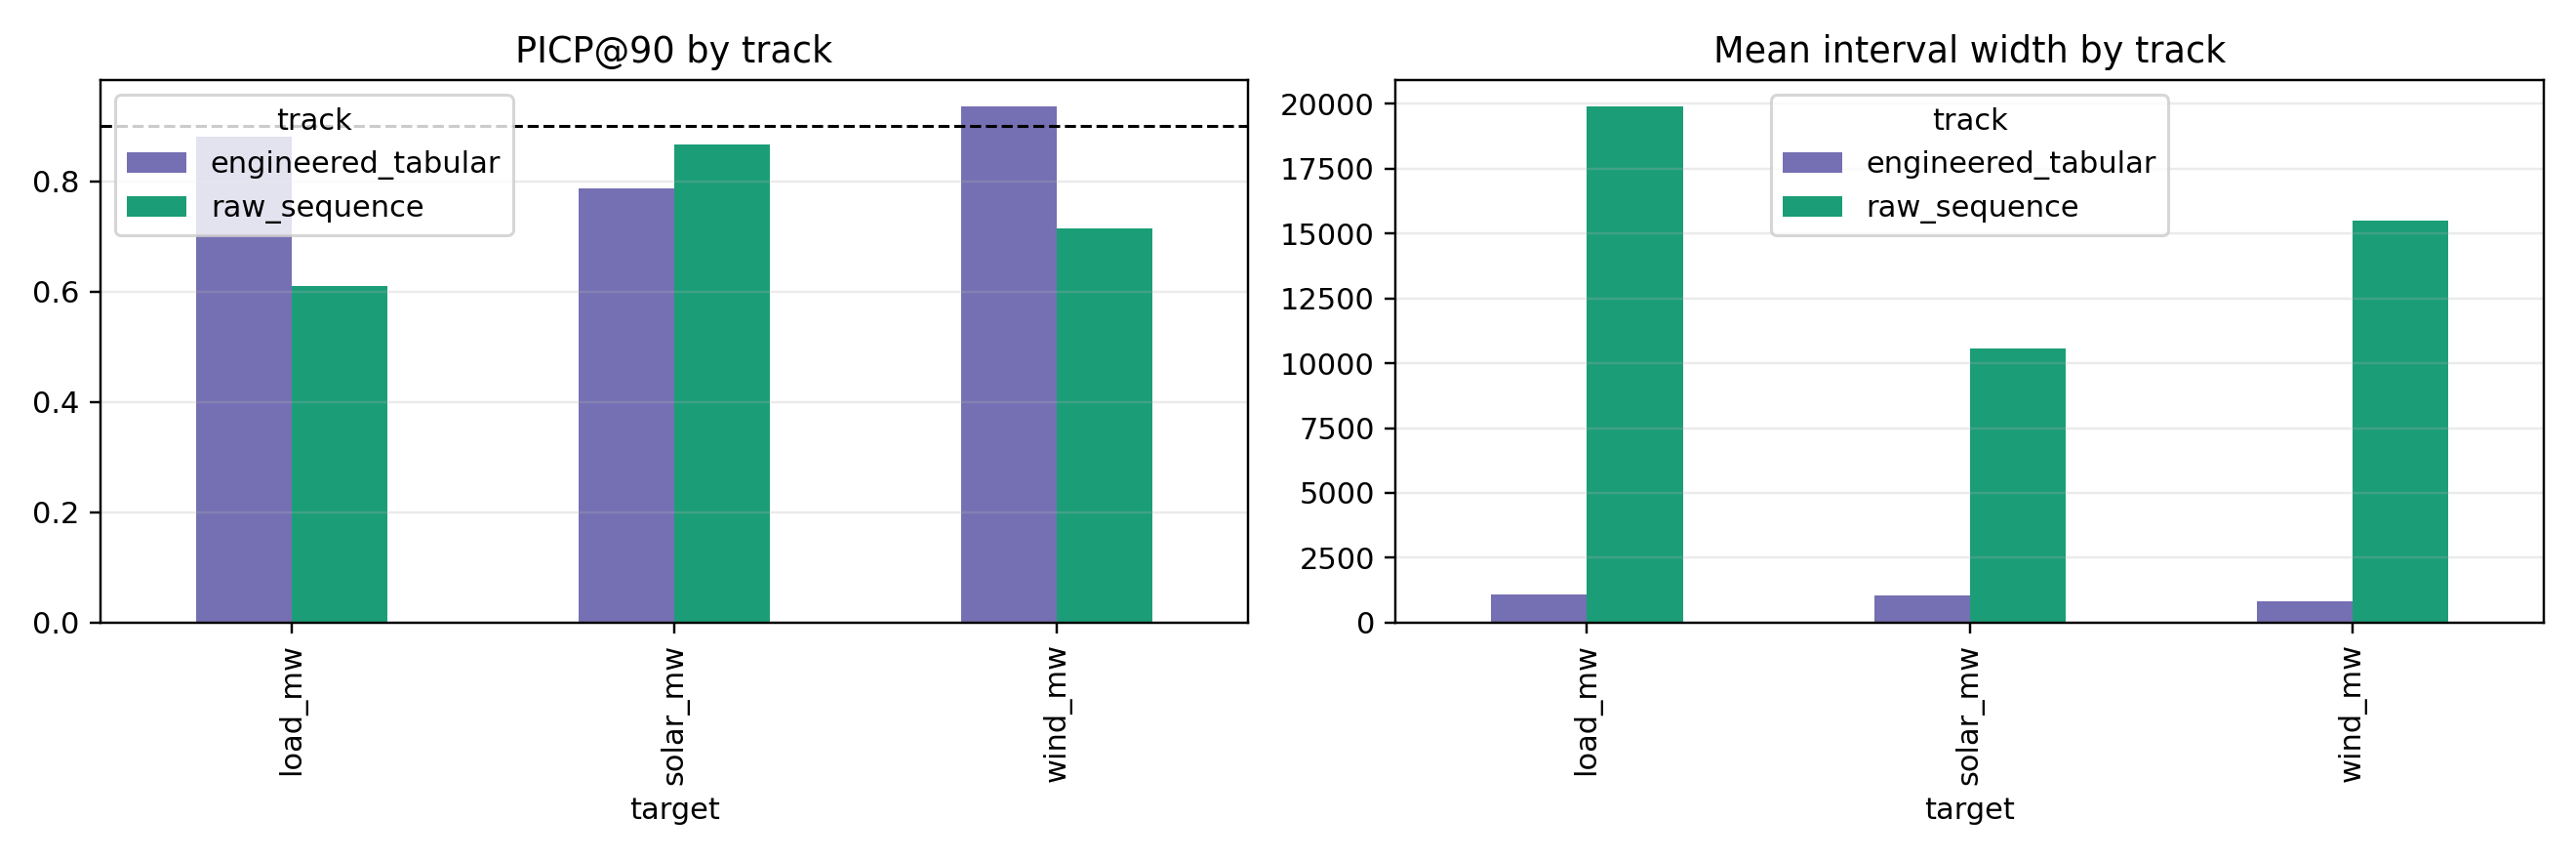
\includegraphics[width=\linewidth]{fig_battery_raw_sequence_track_benchmark}
\caption{Raw-sequence track benchmark from the locked publication package.  The
benchmark is intentionally hard: the raw-sequence model is materially worse
than the engineered baseline, which is why ORIUS treats this track as a
stress-test rather than a victory lap.}
\label{fig:prof-raw-seq-benchmark}
\end{figure}

\subsection{Operational trace and failure analysis}
The 48-hour operational trace and the ablation suite give the strongest
mechanistic evidence.  In the trace, interventions cluster around telemetry
degradation rather than random dispatch variation, and the shield is otherwise
transparent.  In the ablation study, disabling OQE, inflation, or projection
reduces the quality of the protection layer; disabling FTIT mostly increases
conservatism rather than breaking safety.

\begin{itemize}
  \item The 48-hour trace records 47 interventions over 1\,680 steps, or 2.8\%
  of steps, with clusters tied to dropout bursts and drift peaks.
  \item The most severe avoided violation in the trace occurs when the LP
  proposes a large discharge against an over-optimistic observed SOC, while the
  shield projects the action back to a safe discharge.
  \item The ablation tables show that OQE and uncertainty inflation are the
  safety-critical elements; FTIT is a performance refinement, not the main
  safety barrier.
\end{itemize}

\noindent This is the right level of detail for the professor-facing manuscript:
the safety story is not a single lucky run, but a reproducible pattern across
controller rankings, reliability audits, raw-sequence stress tests, and trace-level
failure avoidance.

\ORIUSReuseInput{../monograph/ch07_system_benchmark_governance.tex}
\ORIUSReuseInput{../../chapters/ch22_latency_systems_footprint.tex}
\ORIUSReuseInput{../../chapters/ch30_orius_bench_battery_track.tex}
\ORIUSReuseInput{../../chapters/ch32_certos_runtime_certificate_lifecycle.tex}
\ORIUSReuseInput{../../appendices/app_t_certos_artifact_audit.tex}
\ORIUSReuseInput{../../appendices/app_u_certos_lifecycle_log.tex}
\ORIUSReuseInput{../monograph/app_af_domain_protocol_cards.tex}

\end{document}
